%!TEX root = ./template-skripsi.tex
%-------------------------------------------------------------------------------
%                            BAB III
%               			PEMBAHASAN
%-------------------------------------------------------------------------------

\chapter{METODOLOGI PENELITIAN}

Berikut adalah diagram alir dari penelitian yang akan penulis lakukan :

\begin{figure}[H]
	\centering{}
	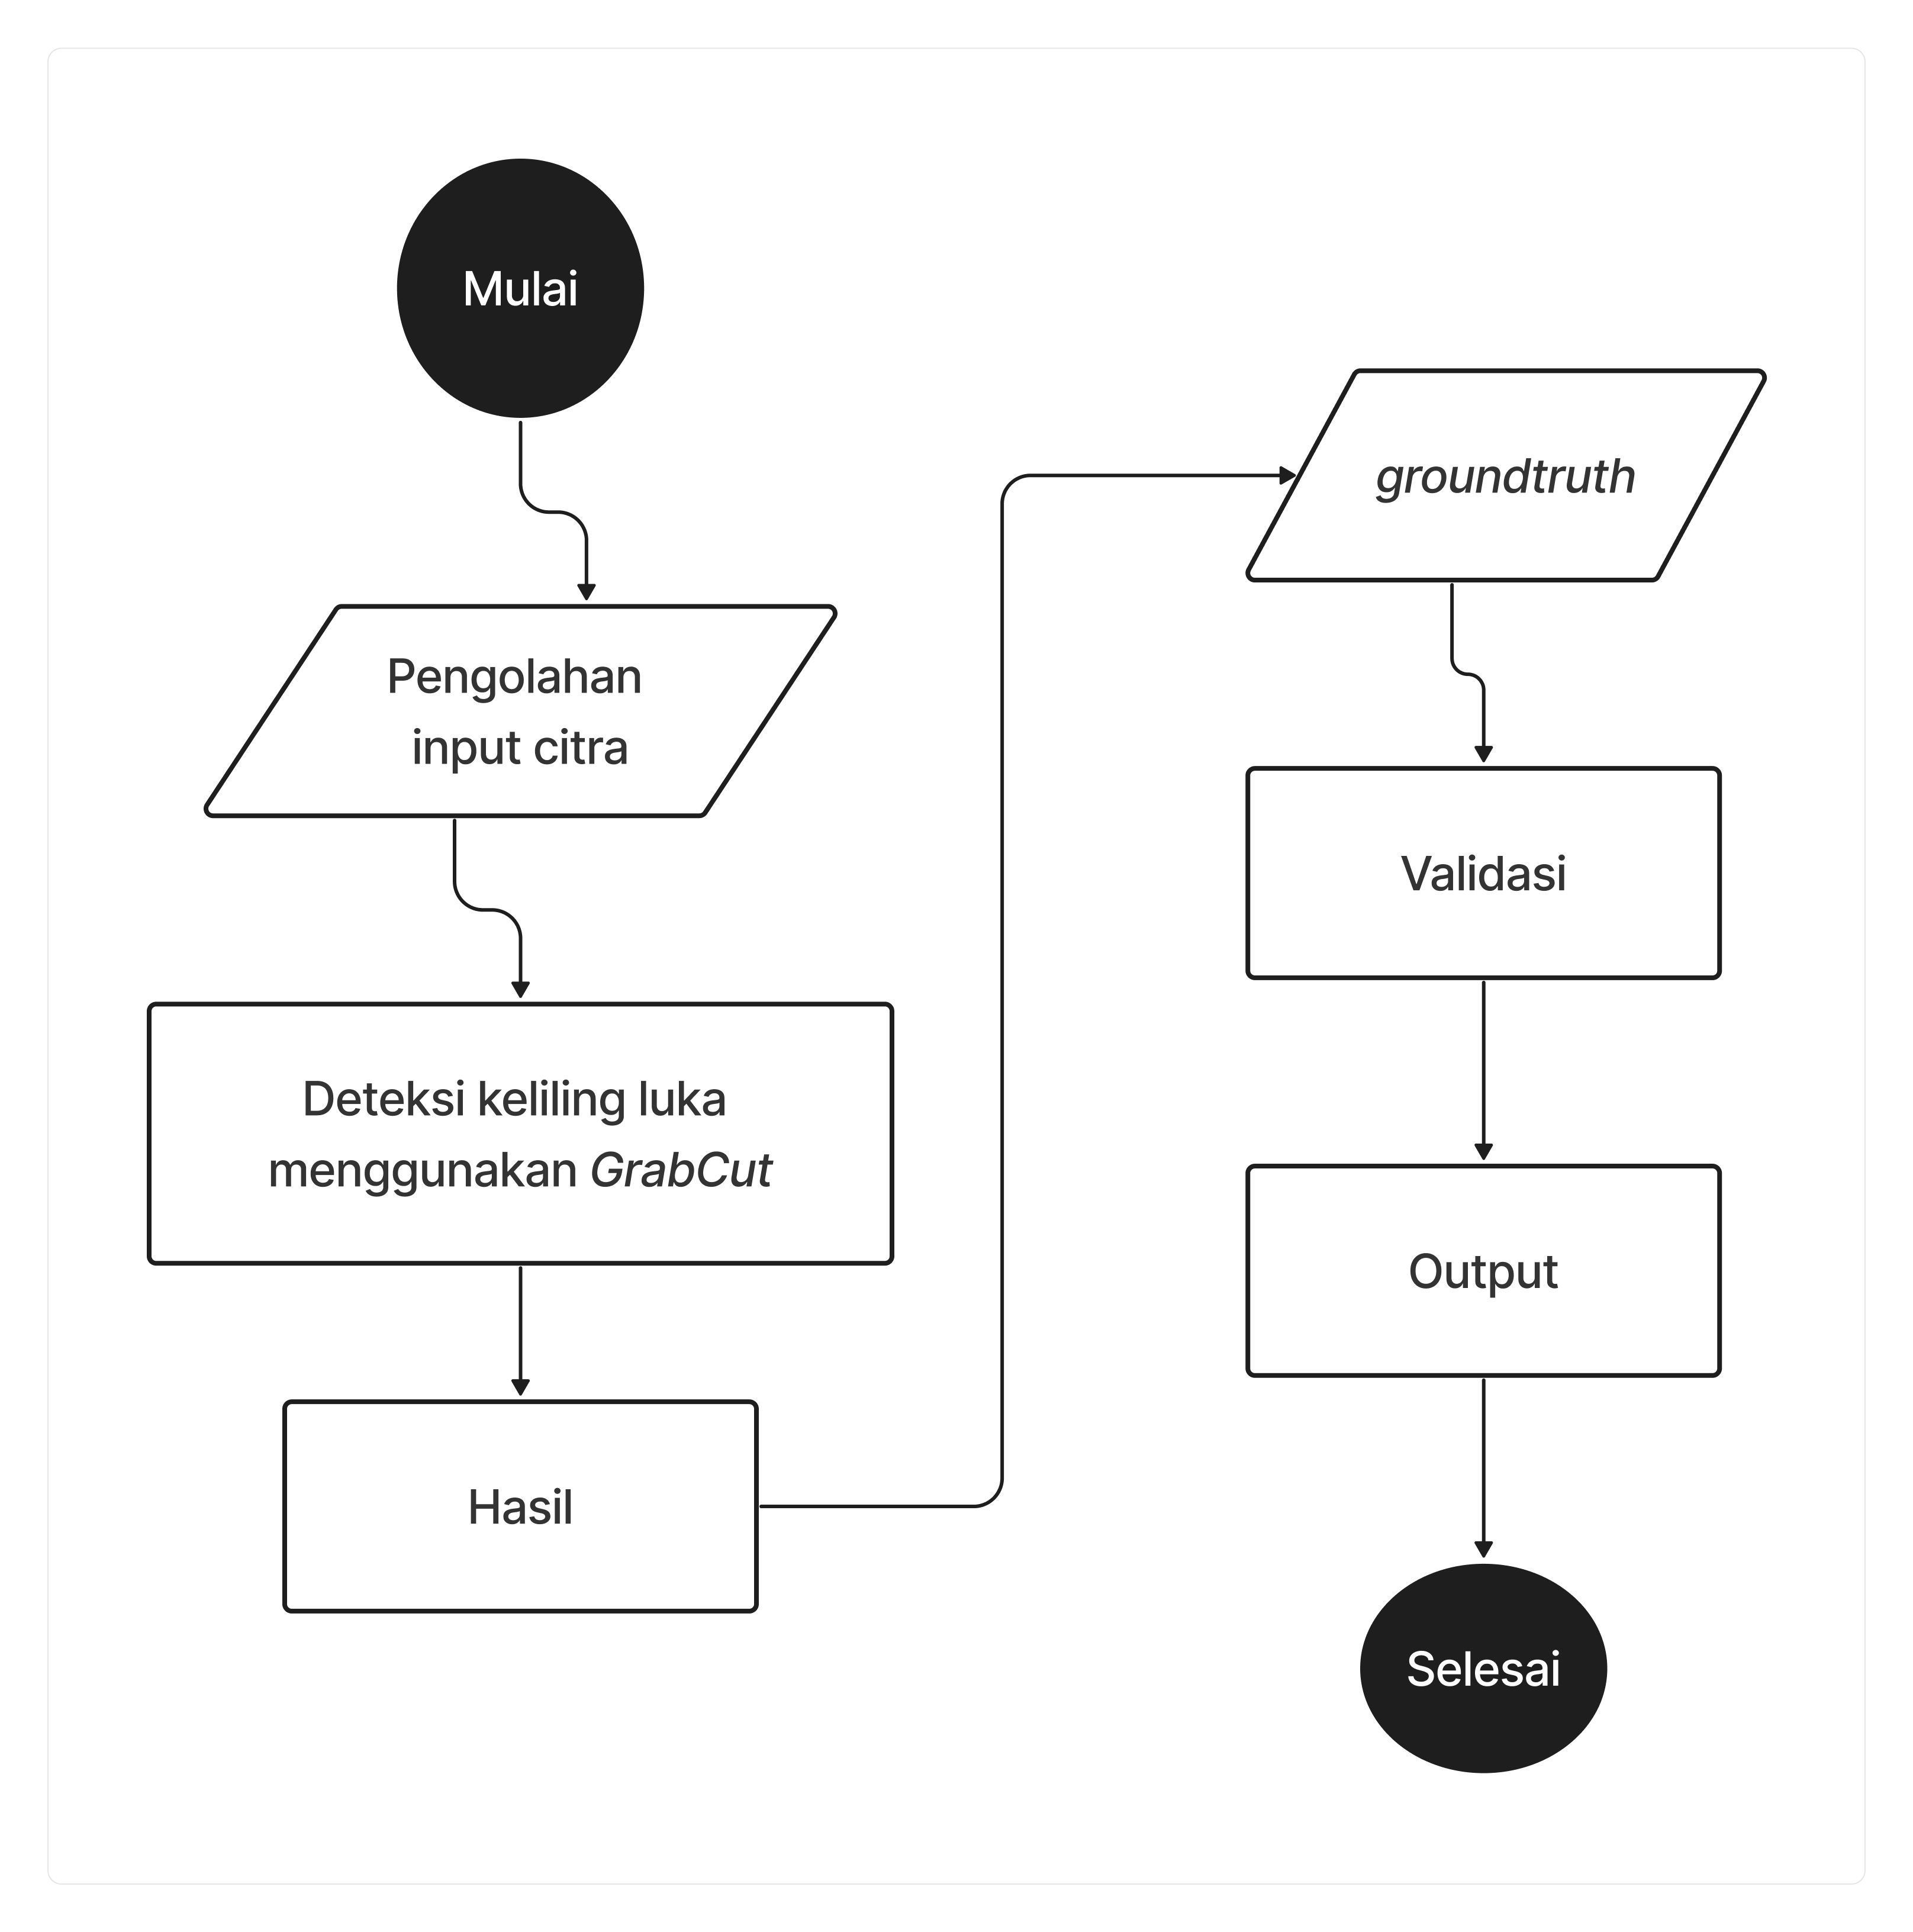
\includegraphics[width=0.8\textwidth]{gambar/gambar-3_1.png}
	\caption{Diagram alir keseluruhan penelitian}
  \end{figure}

\section{Pengolahan \emph{dataset} input citra}

Sebelum melakukan inisiasi pada luka, penulis perlu menyiapkan \emph{dataset} luka, \emph{dataset}
ini kemudian penulis jadikan sampel data input citra. Sampel data dinilai baik 
ketika sampel tersebut mencerminkan populasi dari data tersebut (\cite{Rizki:2022}). 
Silva menggunakan 105 citra luka tentang segmentasi luka otomatis dengan menggunakan 
SVM dan Grabcut(\cite{Silva:2015}). Dalam penelitiannya Wang melakukan automasi segmentasi luka dengan
\emph{Deep Convolutional Neural Networks} menggunakan 2700 citra gambar luka (\cite{Wang:2015}).

Penulis menggunakan \emph{dataset} berjumlah 108, 37 data tidak dapat digunakan 
karena terdapat duplikasi dengan data lain sehingga tersedia 71 buah citra 
yang penulis jadikan sebagai populasi sekaligus sampel (sampel = populasi),
citra tersebut memiliki kategori sesuai dengan warna luka, yaitu luka hitam sebanyak
24 citra, luka kuning sebanyak 15 citra, dan luka merah 32 citra. \emph{Dataset}
penulis dapat dari penelitian luka Ns. Ratna Aryani, K.Kep, tahun 2018 (\cite{Aryani:2018})
yang terdapat pada repositori \url{https://github.com/mekas/InjuryDetection}.

Data awal yang penulis dapat adalah data-data yang berekstensi .xcf yang bisa 
dibuka menggunakan \emph{software} GIMP, pengolahan data sebelum deteksi menggunakan
\emph{GrabCut} dilakukan menggunakan \emph{software} Figma. Masing-masing \emph{dataset} 
didalamnya terdapat \emph{layer} citra (luka), \emph{layer} region (luka), dan 
\emph{path} sebagai berikut :

\begin{figure}[H]
	\centering
	  \begin{subfigure}{0.2\textwidth}
		\centering{}
		
\includegraphics[width=\textwidth]{gambar/gambar-3_2(a).png}
		\caption{}
	  \end{subfigure}%
	  \begin{subfigure}{0.2\textwidth}
		\centering{}
		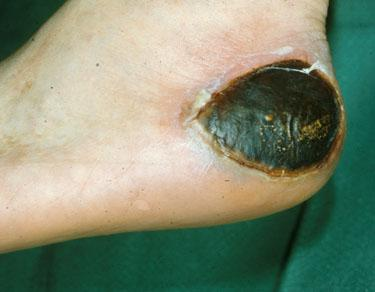
\includegraphics[width=\textwidth]{gambar/gambar-3_2(b).jpg}
		\caption{}
	  \end{subfigure}  
	  \begin{subfigure}{0.2\textwidth}
		\centering{}
		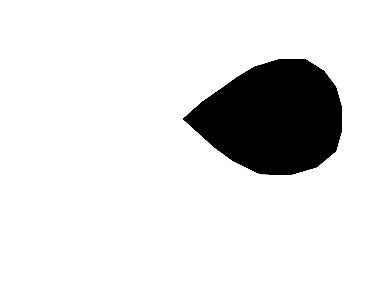
\includegraphics[width=\textwidth]{gambar/gambar-3_2(c).jpg}
		\caption{}
	  \end{subfigure}
	  \begin{subfigure}{0.2\textwidth}
		\centering{}
		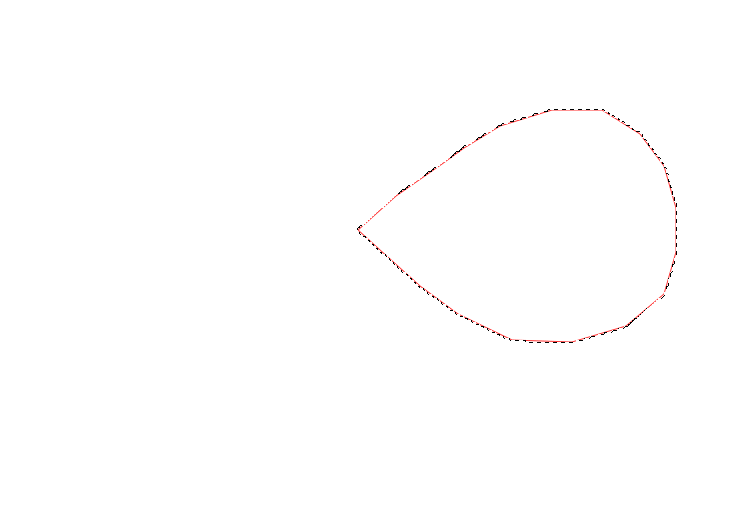
\includegraphics[width=\textwidth]{gambar/gambar-3_2(d).png}
		\caption{}
	  \end{subfigure}  
	\caption{
		(a)Data citra format .xcf, (b) \emph{layer} citra (luka), (c) \emph{layer} 
		region, (d)path
	 }
  \end{figure}

Langkah selanjutnya adalah penulis memasukkan data citra 2(b) ke dalam figma untuk
membuat \emph{layer} dan region (luka) dengan menggunakan \emph{pen tools}, hasil 
dari \emph{pen tools} akan berupa \emph{stroke} atau seperti path 2(d), kemudian 
penulis menduplikasi hasil path dan mengubahnya menjadi objek (\emph{fill object})
seperti 2(c).


\begin{figure}[H]
	\centering{}
	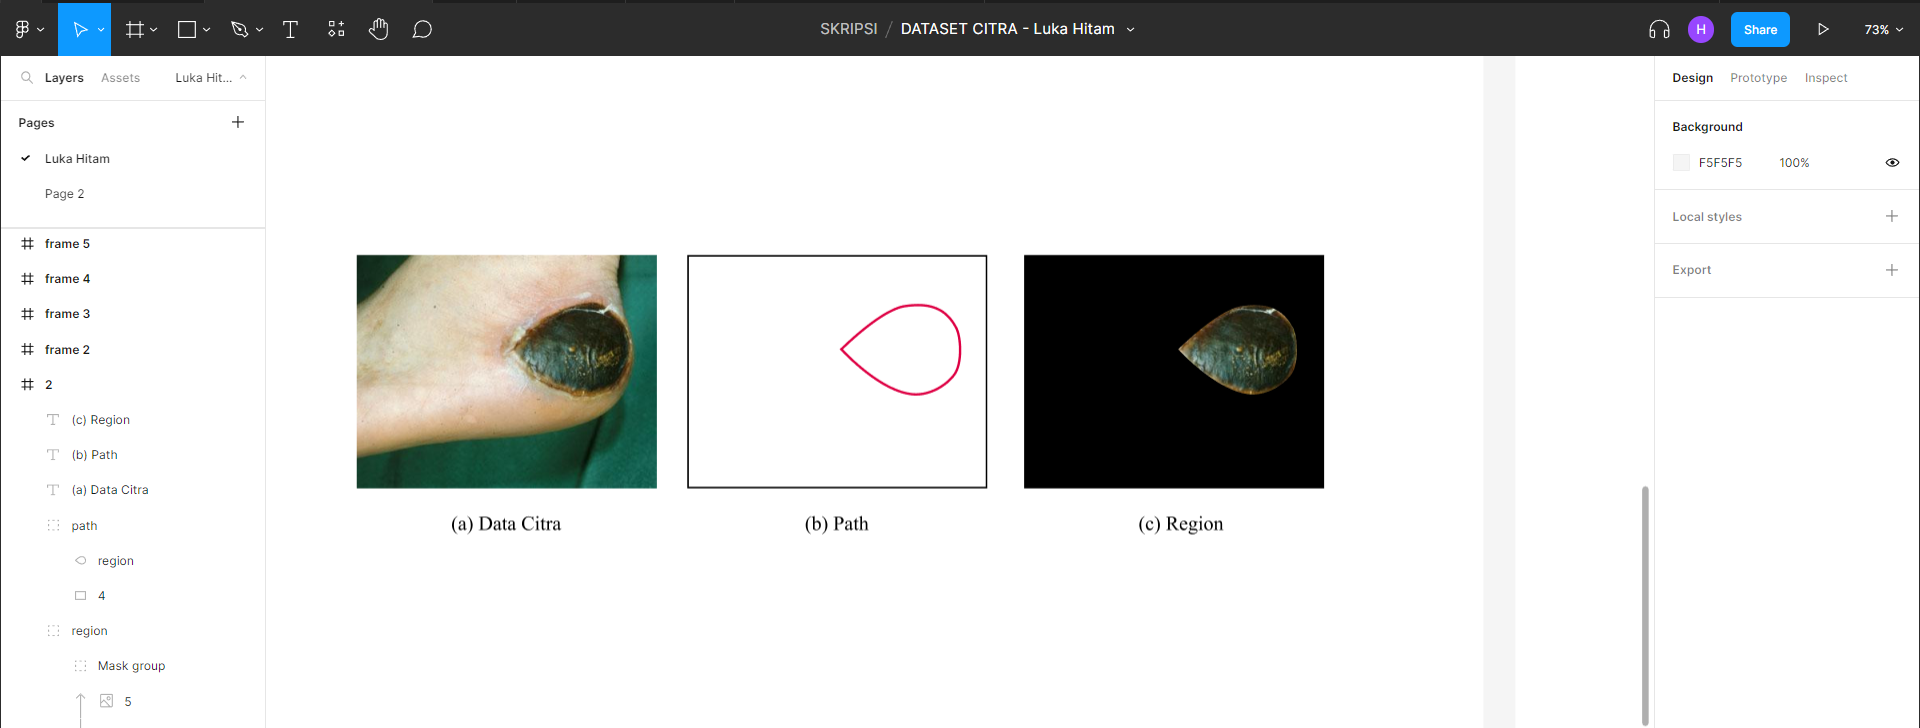
\includegraphics[width=\textwidth]{gambar/gambar-3_3.png}
	\caption{Pengolahan data citra dengan figma}
  \end{figure}

Penulis melanjutkan pengolahan data citra dengan mengubah ukuran (\emph{resize})
citra dengan ukuran yang lebih kecil sehingga tidak lebih dari 2 \emph{megabyte} 
agar proses segmentasi nanti menjadi lebih cepat. Penulis mengubah ukuran citra 
menggunakan fitur \emph{export} dari figma sebesar 0.5 dari ukuran awal citra.

\begin{figure}[H]
	\centering{}
	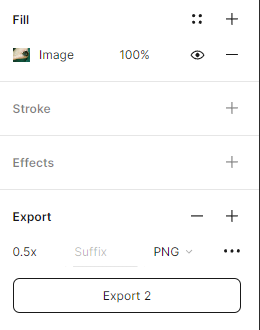
\includegraphics[width=0.3\textwidth]{gambar/gambar-3_4.png}
	\caption{Proses \emph{resize} citra gambar luka dengan ukuran 0.5 dari ukuran awal}
  \end{figure}

Setelah penulis melakukan \emph{resize} ukuran citra, selanjutnya penulis \emph{export}
\emph{layer} masing masing ke format .jpg.

  \begin{figure}[H]
	\centering{}
	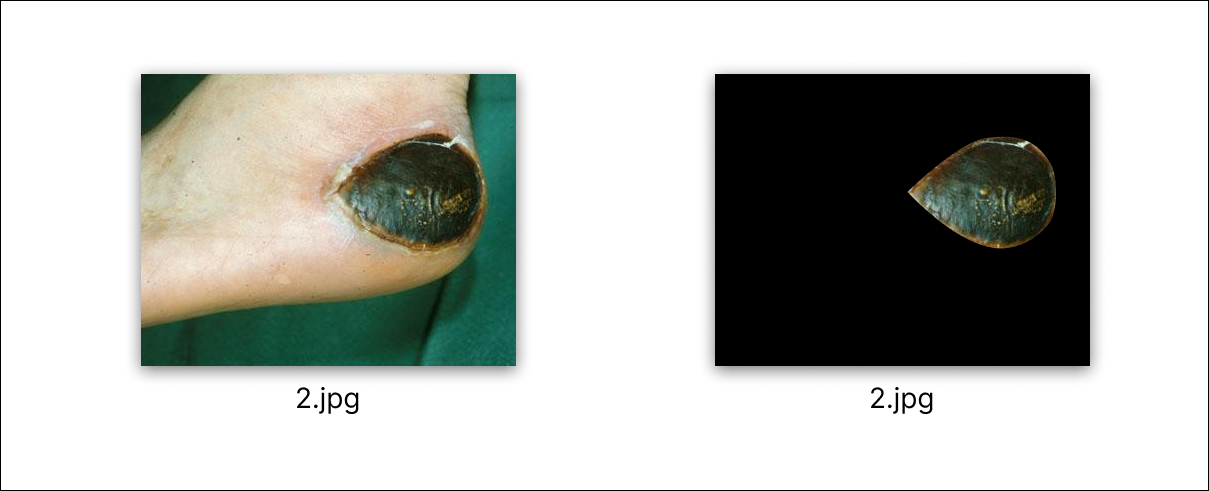
\includegraphics[width=\textwidth]{gambar/gambar-3_5.png}
	\caption{Citra gambar luka dan \emph{region} luka}
  \end{figure}


\section{Segmentasi gambar luka menggunakan \emph{GrabCut}}

Penulis lanjutkan dengan segmentasi citra luka menggunakan \emph{GrabCut}. Segmentasi
citra gambar luka yang penulis lakukan dalam penelitian ini adalah untuk memisahkan
objek luka dengan latar belakangnya pada citra digital, proses segmentasi citra menggunakan
\emph{GrabCut} dilakukan dengan beberapa tahapan. 

\subsection{Inisiasi \emph{Bounding Box}}
Penulis melakukan inisiasi \emph{bounding box} pada daerah yang melingkupi objek 
dimana daerah yang berada didalam \emph{bounding box} akan digunakan untuk membuat 
Trimap \((T_{U})\) dan daerah di luarnya akan dianggap sebagai \emph{background} 
atau \((T_{B})\). Setiap piksel-n yang termasuk \((T_{B})\) akan memiliki \(\alpha_{n}\) 
bernilai 0, sedangkan piksel-n dari \((T_{U})\) akan bernilai 1 untuk \(\alpha_{n}\) nya. 
Tujuan dari \emph{bounding box} ialah untuk mempercepat waktu komputasi dari 
algoritma serta meningkatkan tingkat akurasi segmentasi.

\begin{figure}[H]
	\centering{}
	\includegraphics[width=0.8\textwidth]{gambar/gambar-3_6.png}
	\caption{Diagram alir segmentasi citra gambar dengan metode algoritma \emph{GrabCut}}
\end{figure}


\subsection{Deteksi Objek Citra dengan GMM}

\emph{Gaussian Mixture Model} (GMM) adalah model probabilistik yang dipakai untuk
menggambarkan distribusi probabilitas sebuah kumpulan populasi, GMM mengasumsikan 
bahwa populasi tersebut terdiri dari \emph{mixture} yang berbeda, setiap \emph{mixture} 
diasumsikan mengikuti distribusi normal dan memiliki parmeter yang berbeda. 
Setiap \emph{mixture} bisa kita representasikan dengan \(k \in \{1, ..., K\}\), 
dimana \(K\) adalah total \emph{mixture} yang ada. Setiap gaussian pada \(k\) terdiri dari 
beberapa parameter di antaranya sebagai berikut :

\begin{enumerate}
	\item Rata-rata \(\mu\) yang menginterpretasikan posisi titik puncak dari kurva
	\item Matriks kovarians \(\Sigma\) yang menginterpretasikan sebagai lebar kurva
	\item Probabilitas prior \(\omega\) merupakan peluang sebuah data berasal dari 
		  suatu \emph{mixture} tertentu dengan jumlah maksimal sama dengan 1
\end{enumerate}

Penulis membuat ilustrasi dari parameter gaussian dalam bentuk kurva yang berdistribusi 
normal dalam satu dimensi:

\begin{figure}[H]
	\centering{}
	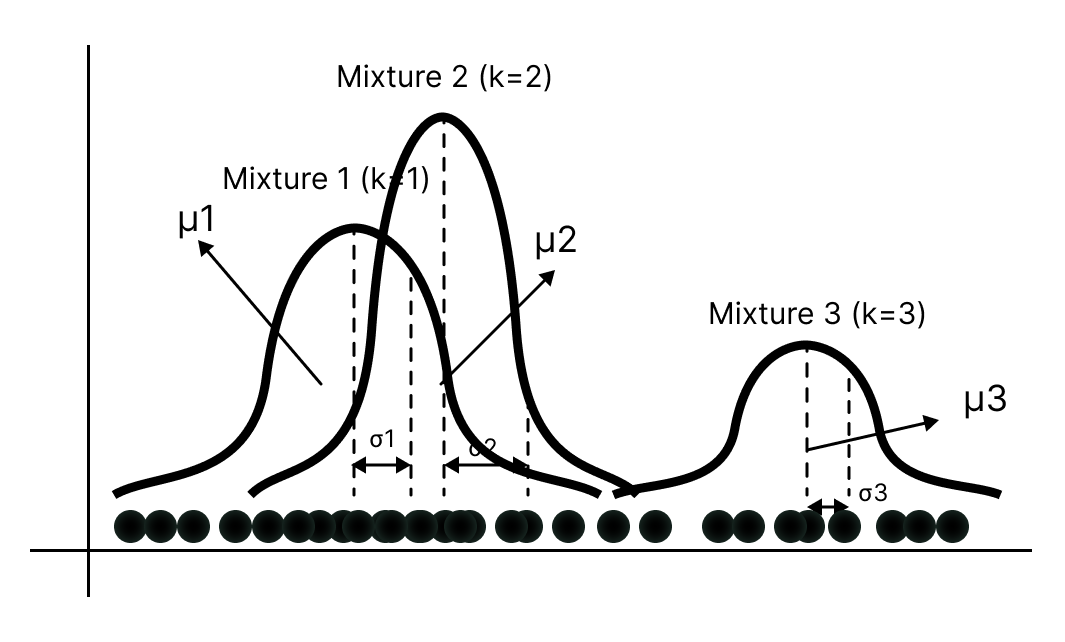
\includegraphics[width=0.8\textwidth]{gambar/gmm_curve.png}
	\caption{Tiga fungsi gaussian dengan parameter K = 3}
\end{figure}

Terlihat bahwa terdapat tiga fungsi gaussian, dengan parameter K = 3. Setiap gaussian
menjelaskan data-data yang terdapat pada tiga \emph{mixture} yang ada. 

\subsubsection{Inisiasi GMM}

Pertama penulis akan melakukan inisiasi untuk tiap parameter GMM, di antaranya 
\(\{\mu, \Sigma \}\), pada algoritma \emph{grabcut} akan digunakan K = 5. Adapun
inisiasi yang dilakukan adalah membuat nilai random terhadap \(\mu\) dan \(\Sigma\).
setelah itu penulis menentukan \(\omega_k = \frac{1}{5}\), untuk \(k \in \{1, ..., 5\}\).
Distribusi gaussian yang akan digunakan untuk citra gambar berwarna yaitu distribusi 
gaussian \emph{multivariate} 2 dimensi atau 3 dimensi, sebagai ilustrasi gausian berdistribusi 
normal 2 dimensi dengan objek citra gambar luka berwarna :

\begin{figure}[H]
	\centering
	  \begin{subfigure}{0.4\textwidth}
		\centering{}
		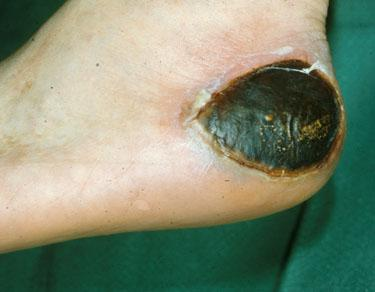
\includegraphics[width=\textwidth]{gambar/gambar-3_2(b).jpg}
		\caption{}
	\end{subfigure}\hfill% or \hspace{5mm} or \hspace{0.3\textwidth}
	  \begin{subfigure}{0.4\textwidth}
		\centering{}
		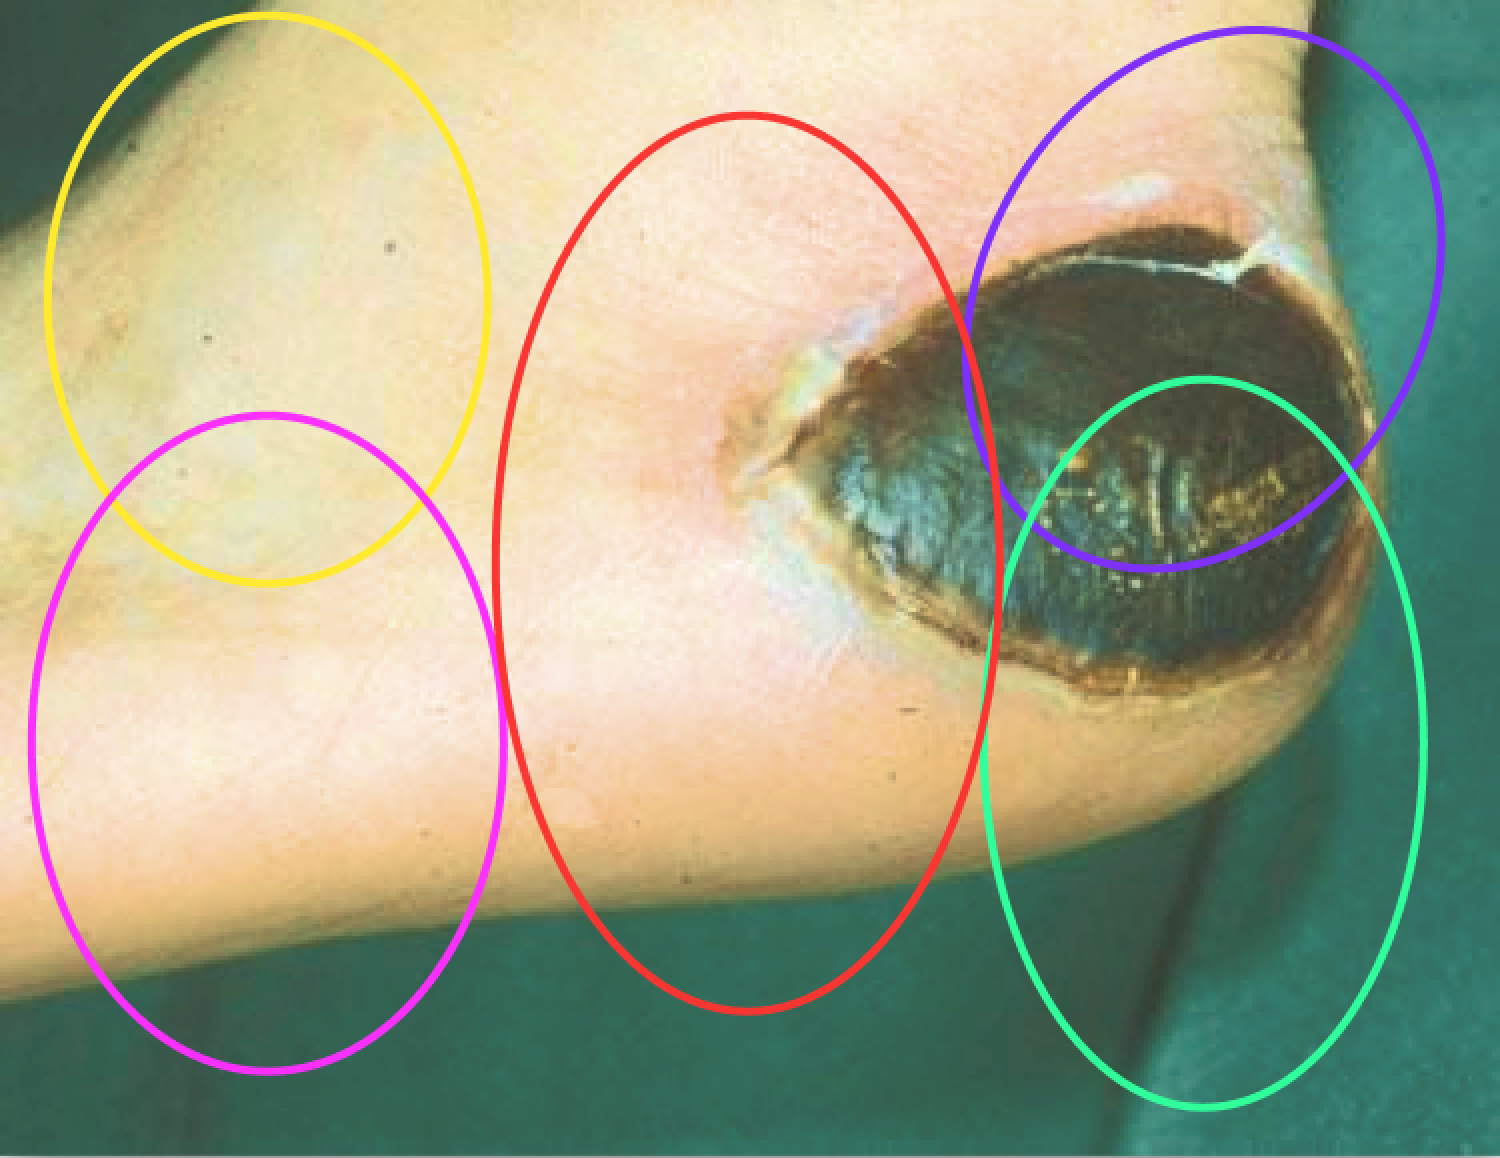
\includegraphics[width=\textwidth]{gambar/gambar-3_7.png}
		\caption{}
	  \end{subfigure} 
	\caption{
		(a) Citra gambar luka, (b) Deteksi \emph{clustering} citra dengan GMM
	 }
  \end{figure}

Prior probabilitas harus memenuhi kondisi :

\begin{equation} \label{}
	\Sigma^K_{k=1} \omega_k = 1
\end{equation}

Secara umum rumus distribusi gaussian didefinisikan sebagai berikut :

\begin{equation} \label{}
f(x) = \frac{1}{\sigma \sqrt{2\pi}} e^{-0.5 \bigl(\frac{x - \mu}{\sigma} \bigr)^2}
\end{equation}

Persamaan di atas merupakan rumus dari distribusi normal (gaussian) untuk 1 dimensi, 
dimana parameter yang digunakan adalah standar deviasi (\(\sigma\)). Sedangkan 
untuk distribusi gaussian n-dimensi maka digunakan persamaan berikut :


\begin{equation} \label{}
	f_{X|k} (X|k, \theta_k) = \frac{1}{(2\pi)^\frac{n}{2} |\Sigma_k|^\frac{1}{2}} e^{-\frac{1}{2} (X - \mu_k)^T \Sigma^{-1}_k (X - \mu_k)}
\end{equation}

\(f_{X|k} (X|k, \theta_k)\) menjelaskan distribusi \emph{mixture} ke-k.Nilai k 
tersembunyi dan dapat diukur secara tidak langsung dengan nilai piksel \(X\) 
dimana \(x\) mencakup nilai dari k. Nilai dari piksel X dapat diasumsikan dengan 
rumus di atas dengan parameter \(\theta_k = \{ \mu_k, \Sigma_k \}\)

Karena nilai k saling lepas maka dapat ditentukan distribusi X sebagai jumlah dari
distribusi masing-masing \emph{mixture} yaitu :

\begin{equation} \label{}
	f_{X}(X|\Phi) = \Sigma_{k=1}^K \omega_k f_{X|k} (X|k,\theta_k)
\end{equation}

Pendugaan parameter dapat dilakukan dengan menggunakan algoritma \emph{expectation-maximization} (EM).
Langkah pertama dari algoritma EM adalah dengan mengestimasi nilai \(P(k|X,\Phi)\) 
yang dapat dihitung menggunakan teorema Bayes :

\begin{equation} \label{}
	P(k|X,\Phi) = \frac{\omega_k f_{X|k} (X|k,\theta_k)}{f_X(X|\Phi)}
\end{equation}

Dilanjutkan dengan menetapkan nilai \(k\) pada setiap piksel menggunakan rumus :

\begin{equation} \label{eq:3.6}
	\hat{k} = arg \max_{k} P(k|X,\Phi) 
\end{equation}

Adapun dengan memisalkan \(D(k|X,\Phi) = - \log P(k|X,\Phi)\), maka persamaan \ref{eq:3.6}
menjadi seperti langkah pertama pada gambar \ref{gambar:2.6} yaitu sebagai berikut :

\begin{equation} \label{eq:3.6}
	\hat{k} = arg \min_{k} P(k|X,\Phi) 
\end{equation}


Karena \(f_X(X|\Phi)\) independen terhadap nilai k, maka dapat menuliskan kembali
rumus di atas menjadi : 

\begin{equation} \label{}
	\hat{k} = arg \min_{k} \omega_k f_{X|k} (X|k,\theta_k)
\end{equation}

\subsubsection{Mempelajari parameter GMM}

Setelah memperoleh nilai k, selanjutnya menduga parameter GMM menggunakan metode
\emph{maximum likelihood} untuk memaksimumkan fungsi likelihood, dimana rumus 
fungsi likelihood adalah sebagai berikut:

\begin{equation} \label{}
	P(X_1, X_2, ..., X_N, k | \Phi) = \Pi_{t=1}^N \omega_k f_{X|k}(X_t|k,\theta_k)
\end{equation}

Adapun parameter penduga yang memaksimumkan persamaan di atas adalah sebagai berikut :

\begin{equation} \label{}
	\hat{\omega_k} = \frac{1}{N} \Sigma_{t=1}^N P(k|X_t,\Phi)
\end{equation}

\begin{equation} \label{}
	\hat{\mu} = \frac{\Sigma_{t=1}^N X_t P(k|X_t,\Phi)}{\Sigma_{t=1}^N P(k|X_t,\Phi)} 
\end{equation}

\begin{equation} \label{}
	\hat{\Sigma_k} = \frac{\Sigma_{t=1}^N ((X_t - \hat{\mu_k}) \cdot (X_t - \hat{\mu_k})) P(k|X_t,\Phi)}{\Sigma_{t=1}^N P(k|X_t,\Phi)}
\end{equation}

Dengan memisalkan rumus \ref{eq:2.11} dengan \(U = - \log P(X_1, X_2, ..., X_N, k | \Phi)\)
maka didapatkan hasil seperti langkah kedua dari gambar \ref{gambar:2.6} yaitu 
sebagai berikut :

\begin{equation} \label{}
	\hat{\Phi} = arg \min_{\Phi} P(k|X_t,\Phi)
\end{equation}


% Tahap kedua, penulis memasukkan komponen GMM terhadap piksel yang ada didalam 
% \(T_{U}\) dengan persamaan 

% \begin{equation} \label{eq:3.1}
% 	k_{n} := arg \min_{k_{n}} D_{n}(\alpha_{n}, k_{n}, \theta, z_{n})
% \end{equation}

% Kemudian mencari parameter GMM dari himpunan piksel \textbf{z} dengan rumus 

% \begin{equation} \label{eq:3.2}
% 	\underline{\theta} := arg \min_{\theta} U (\underline{\alpha}, \textbf{k}, \underline{\theta}, \textbf{z}) 
% \end{equation}


\subsection{Iterasi dengan Minimisasi}

Selanjutnya penulis melakukan segmentasi dengan menggunakan algoritma \emph{min-cut/max-flow}
atau \emph{GraphCut}. Algoritma ini memvisualisasikan gambar sebagai graf, dan piksel 
sebagai \emph{node} pada graf tersebut, kemudian \emph{GraphCut} bertugas untuk 
segmentasi piksel mana yang termasuk \emph{foreground} dan \emph{background} dengan cara
melakukan \emph{cut} pada graf. Terdapat dua terminal pada graf yaitu terminal \emph{source} s
dan \emph{sink} t, kedua terminal saling terhubung terhadap semua piksel yang ada di graf,
piksel yang masuk ke dalam \emph{source} akan menjadi \emph{foreground} sementara piksel
yang masuk ke dalam \emph{sink} akan menjadi \emph{background}. Setiap \emph{node} 
pada graf memiliki hubungan yang yang disebut \emph{edge}, \emph{edge} akan memiliki arah 
dan bobot, bobot tersebut akan digunakan untuk mencari \emph{mincut} dari graf.


\begin{figure}[H]
	\centering
	  \begin{subfigure}{.5\textwidth}
		\centering{}
		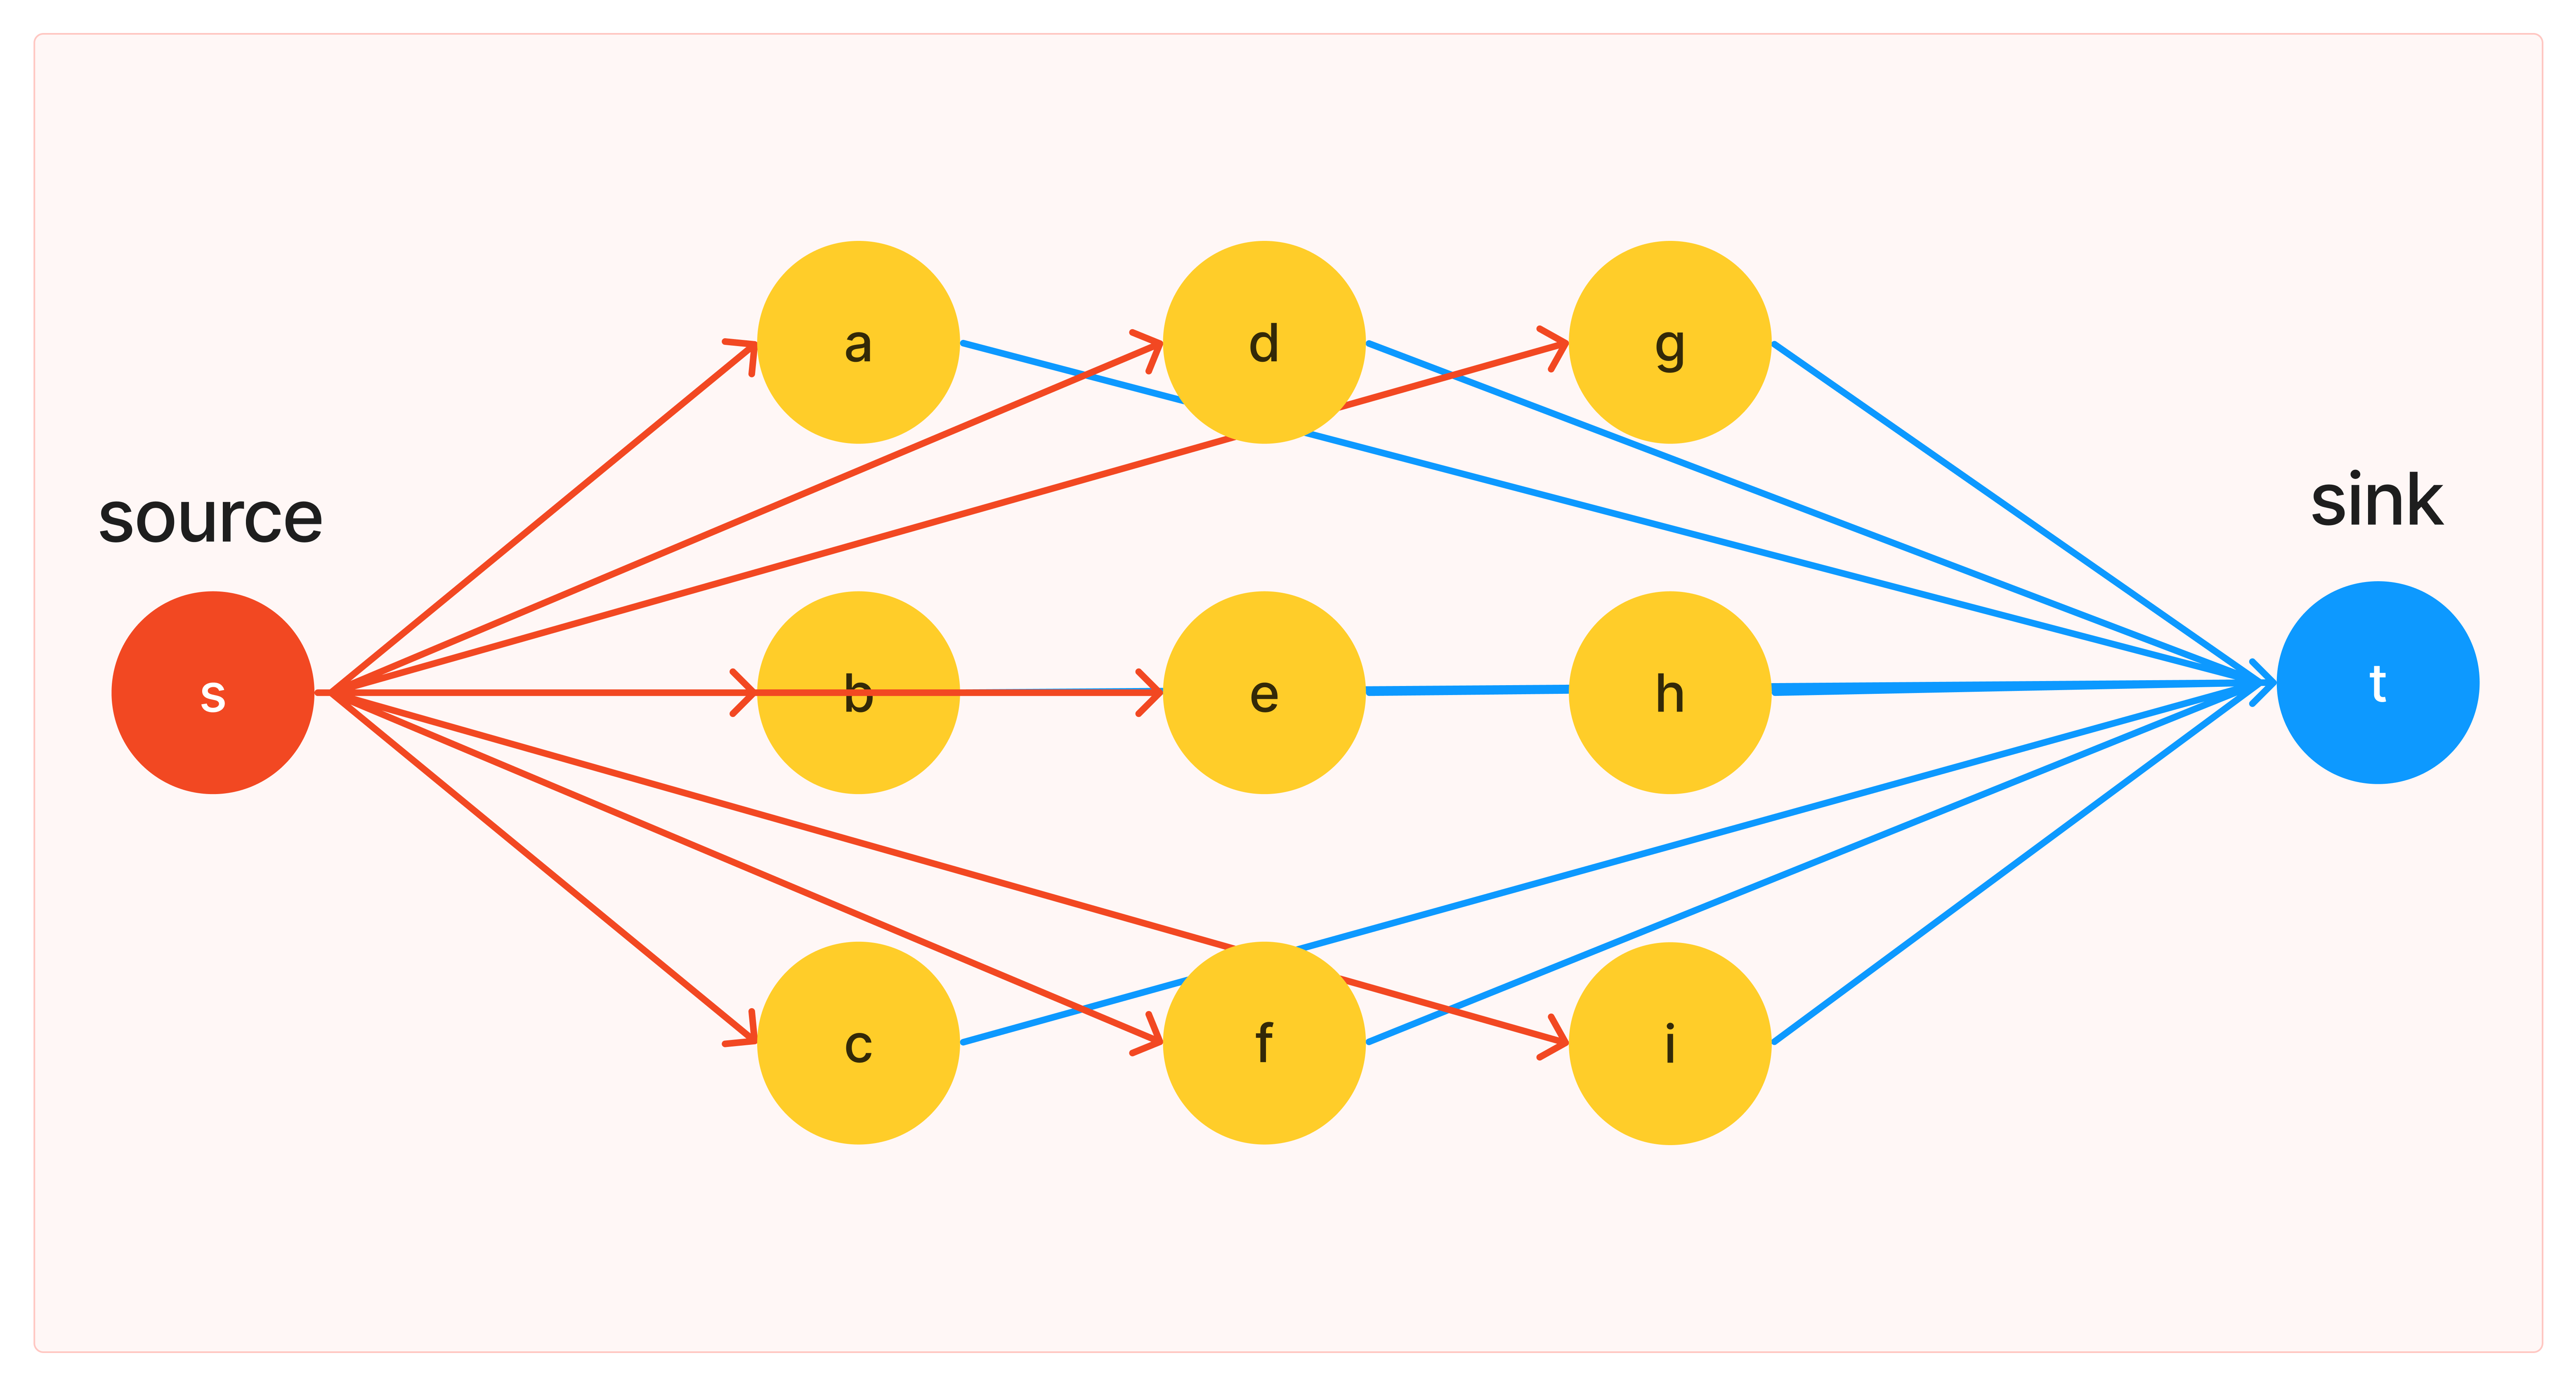
\includegraphics[width=\textwidth]{gambar/cth-graph-1.png}
		\caption{Sebuah graf}
	  \end{subfigure} \hfill
	  \begin{subfigure}{.5\textwidth}
		\centering{}
		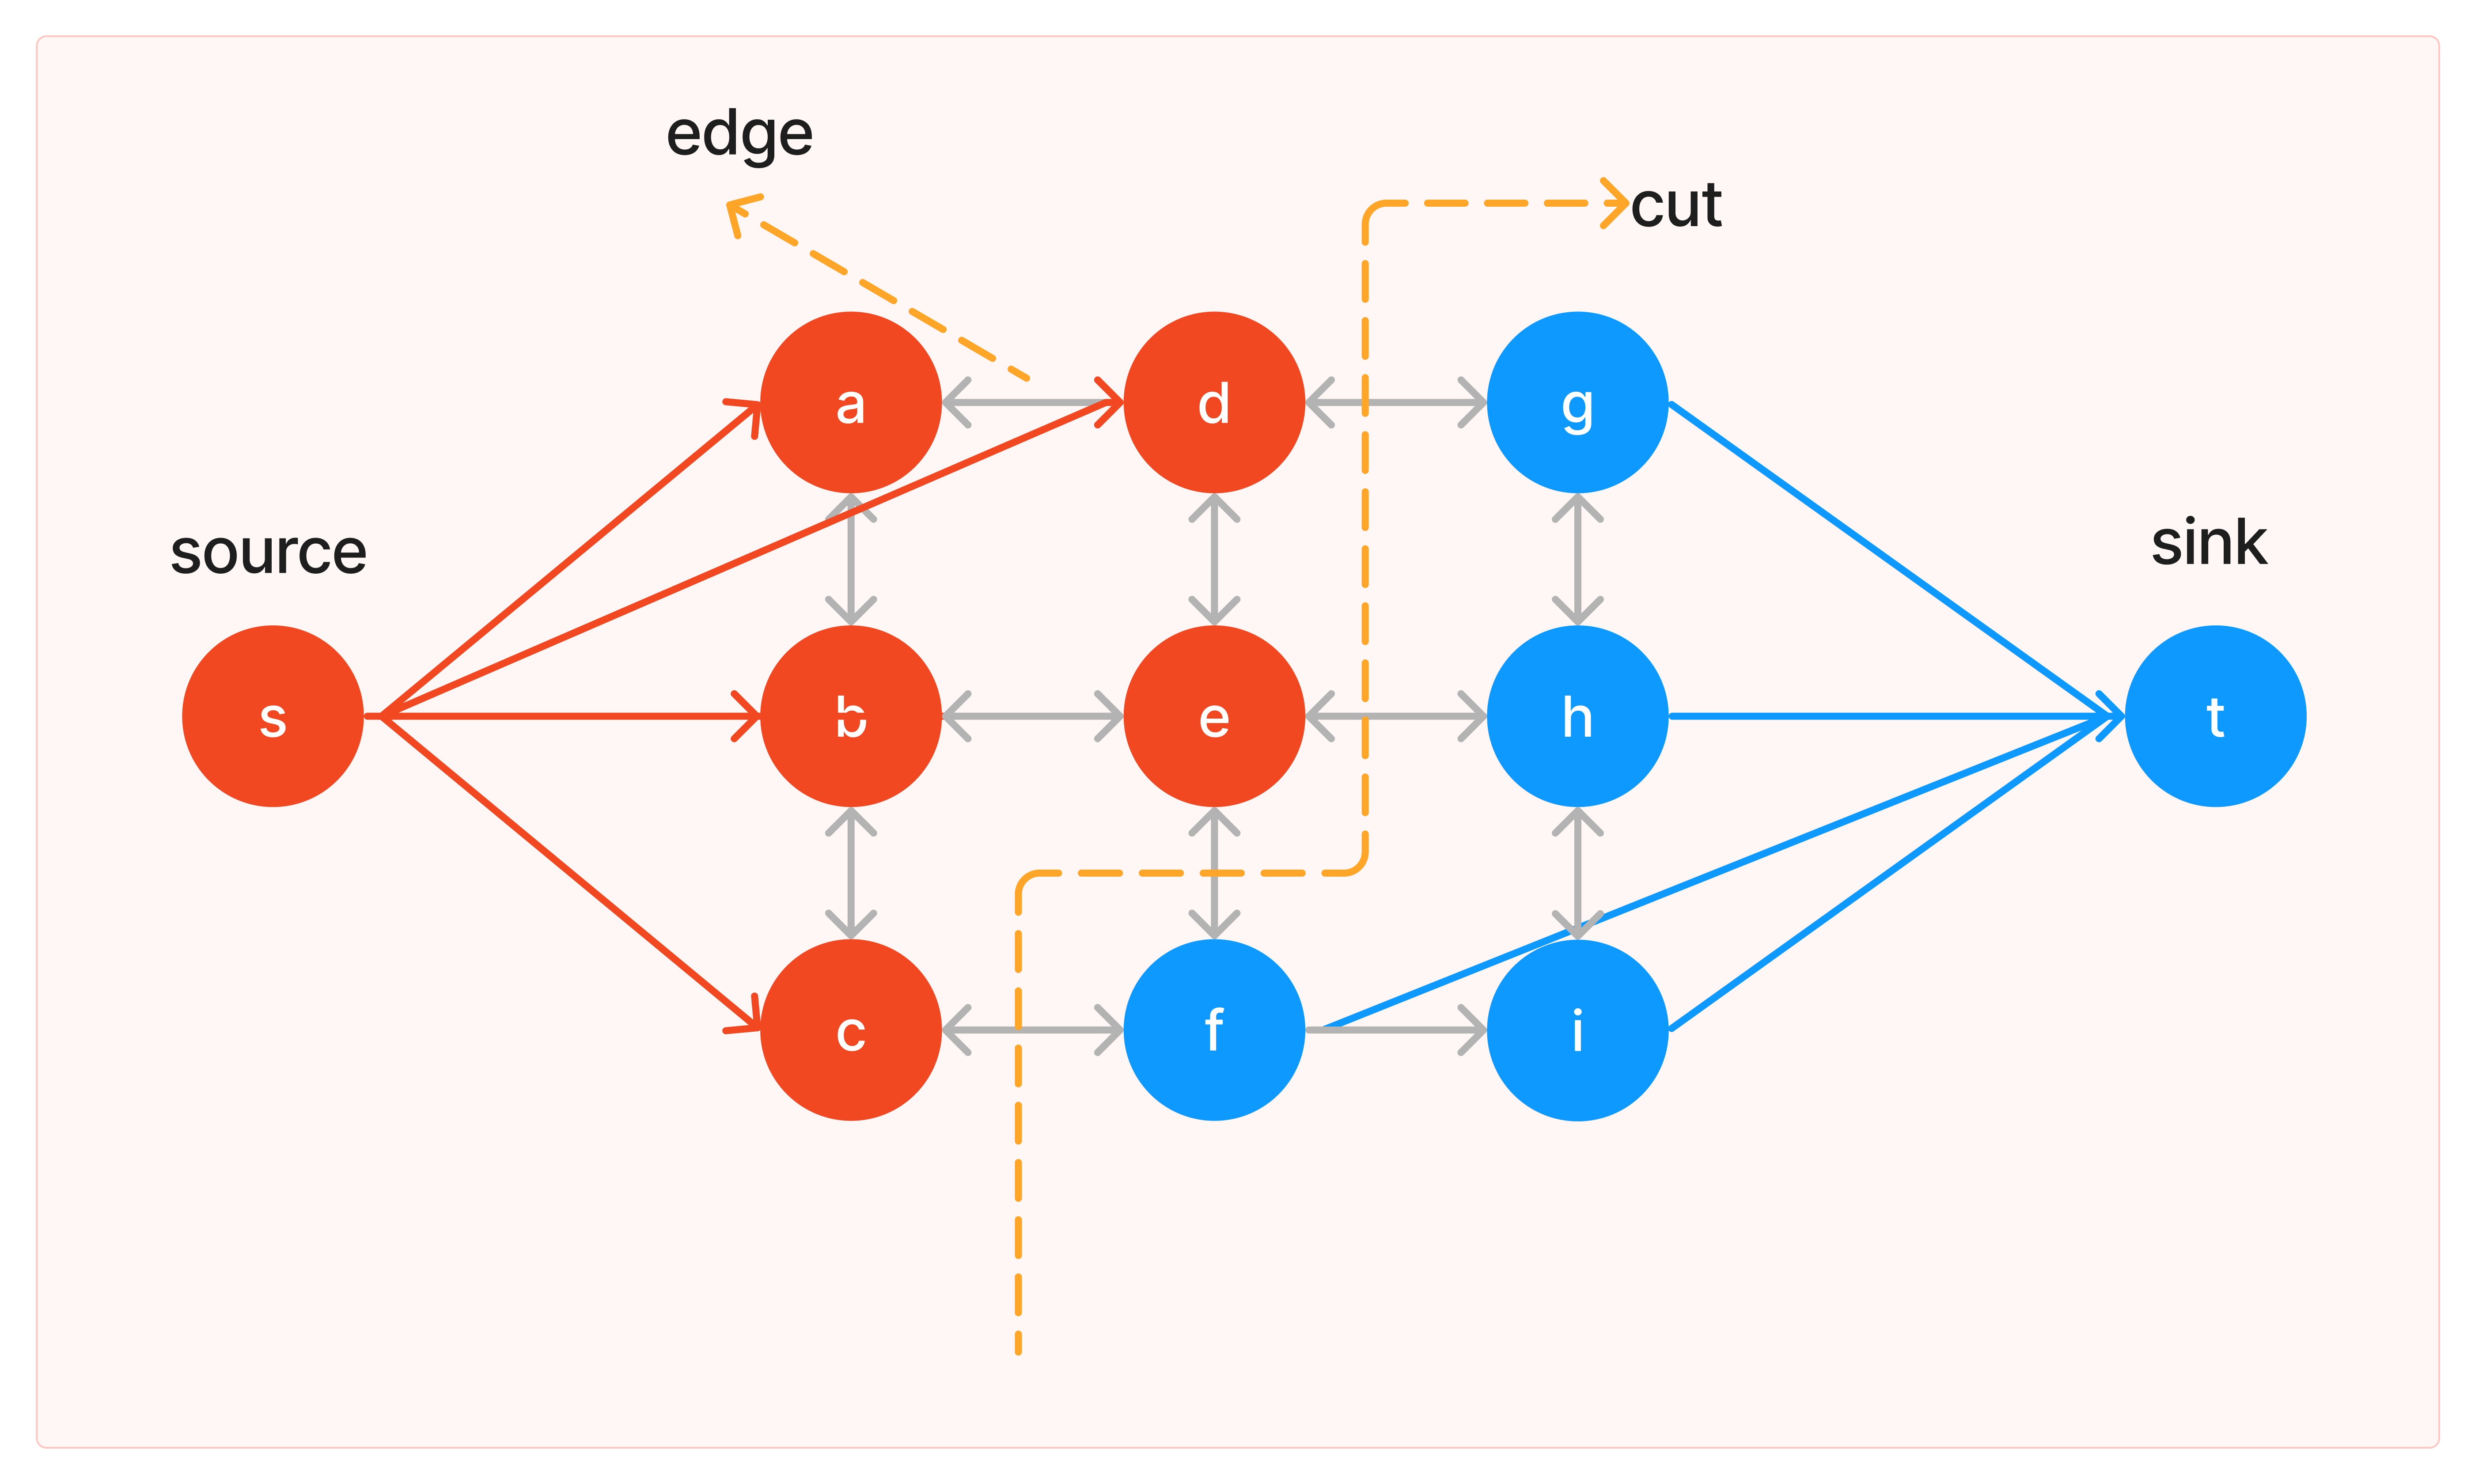
\includegraphics[width=\textwidth]{gambar/cth-graph-2.png}
		\caption{Sebuah (\emph{cut})}
	  \end{subfigure}  
	\caption{
	  Contoh graf berkapasitas terarah.
	  }
	\label{gambar:3.9}
  
  \end{figure}

Algoritma \emph{mincut} terdiri dari beberapa tahap, penjelasan singkatnya yaitu 
tahap pertama dimana graf bertumbuh (\emph{growth}) hingga menemukan jalan (\emph{path}) 
dari \emph{source} menuju \emph{sink}, selanjutnya tahap kedua (augmentasi) dimana 
\emph{path} yang sudah ditemukan akan dilihat kapasitas tiap \emph{edge} nya lalu 
masing-masing kapasitas \emph{edge} akan dikurangi dengan kapasitas paling kecil 
(\emph{bottleneck}), apabila ada kapasitas \emph{edge} yang kosong, maka \emph{node} 
tersebut menjadi \emph{Orphans} (tidak memiliki orang tua), setelah itu masuk tahap 
ketiga (adopsi) yaitu mencari orang tua baru dari \emph{node} yang menjadi \emph{orphans} 
sebelumnya, apabila tidak ada maka \emph{node} tersebut menjadi \emph{node} bebas. 
Struktur algoritma \emph{mincut} dapat dilihat pada bagian \ref{pseudo:1.0}. 

Setiap piksel pada gambar memiliki komponen GMM tersendiri, pada tahap ini nilai k
tiap piksel telah didapatkan dari GMM, dimana nilai k dari tiap piksel memiliki rentang
dari 1 sampai 5. Pada permulaan algoritma \emph{mincut} penulis menentukan \emph{node}
mana yang menjadi tetangga dari \emph{source} atau \emph{sink} dengan menghitung
menghitung jumlah nilai D dari persamaan \ref{eq:2.11} pada setiap komponen GMM, 
kemudian penulis menjumlahkan nilai yang didapat dan membaginya dengan 5 (total K),
nilai yang didapat akan dijadikan sebagai \emph{treshold} dalam menentukan hubungan
tiap piksel ke \emph{Source} atau ke \emph{Sink}.

\begin{lstlisting} [label={pseudo: neighbors_terminals}]
	initialize: (P = [[], [], [], [], []], 
	S = [0,0,0,0,0], 
	G = (V, E), K = Himpunan komponen GMM tiap piksel)
	t = 0
	for every node x $\in$ V : 
		P[K[x]-1] := P[K[x]-1] $\cup$ {x}
		Calculate D for x using $\ref{eq:2.12}$
		S[K[x]-1] += D
	end for

	Calculate t := mean(S)

	for every k $\in$ {1,2,3,4,5}:
	if S[k-1] < t
		E := E $\cup$ (s $\rightarrow$ p) for every p $\in$ P[k-1]
	else
		E := E $\cup$ (p $\rightarrow$ t) for every p $\in$ P[k-1]
	end for

	
  \end{lstlisting}

Selanjutnya masuk ke tahap growth, \emph{augmentation}, dan \emph{adoption}, diagram alir
dari ketiga tahap bisa dilihat sebagai berikut :





% dengan meminimumkan rumus E pada persamaan \ref{eq:2.10}, lalu kembali
% ke langkah awal sampai terjadinya konvergensi yaitu tidak ada perbedaan segmentasi antar Iterasi.

\subsection{Penyuntingan oleh Pengguna}
Langkah selanjutnya penulis melakukan perbaikan dari citra yang sudah di segmentasi
dari hasil sebelumnya dengan menetapkan piksel yang seharusnya menjadi latar belakang
dengan \(\alpha_{n} = 0\), setelah itu kembali pada langkah meminimumkan rumus E yang hanya
dilakukan sekali.

\section{Validasi}
Validasi yang akan penulis lakukan adalah dengan menghitung selisih piksel dari area
segmentasi dengan area \emph{groundtruth} sehingga akan menghasilkan nilai akurasi berikut :
\begin{equation} \label{eq:3.3}
	Akurasi(\%) = 100 - \bigg | \frac{(luas \: area \: groundtruth - luas \: area \: segmentasi)}{luas \: area \: groundtruth} * 100 \bigg |
\end{equation}
